\documentclass[border=1pt]{standalone}
\usepackage{amsmath,amssymb}
\usepackage{pgfplots}
\pgfplotsset{compat=1.18}
\usepgfplotslibrary{groupplots}
\usepackage{pgfplotstable}
\setlength{\textwidth}{5.0in}
\setlength{\linewidth}{5.0in}
\usepackage{xr}
\externaldocument{hyman2026structure_v2_3_0}
\makeatletter
\AtBeginDocument{\@ifundefined{r@sec:integrable-paradigm}{\PackageError{fig_roadmap}{Main-paper labels not found. Compile hyman2026structure_v2_3_0.tex first and put its .aux beside this file}{}}{}}
\makeatother
\begin{document}
\pgfplotstableread[col sep=comma]{figdata/regime_compacton.csv}\regimeA
\pgfplotstableread[col sep=comma]{figdata/regime_solitary.csv}\regimeB
\pgfplotstableread[col sep=comma]{figdata/regime_algebraic.csv}\regimeC
\pgfplotstableread[col sep=comma]{figdata/regime_cnoidal.csv}\regimeD
\pgfplotstableread[col sep=comma]{figdata/profile_compacton.csv}\compactondata
\pgfplotstableread[col sep=comma]{figdata/profile_a0.01.csv}\profileAA
\pgfplotstableread[col sep=comma]{figdata/profile_a0.10.csv}\profileAB
\pgfplotstableread[col sep=comma]{figdata/profile_a0.50.csv}\profileAC
\pgfplotstableread[col sep=comma]{figdata/profile_a1.00.csv}\profileAD
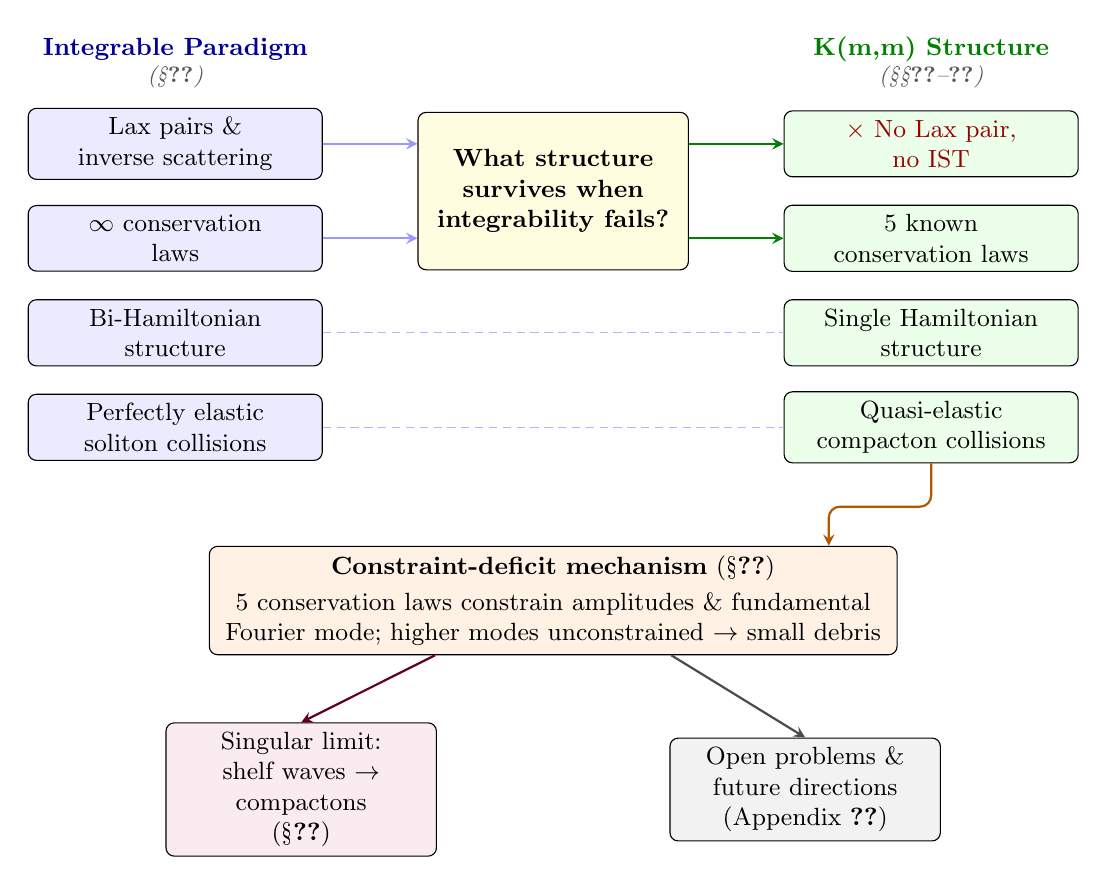
\begin{tikzpicture}[
  box/.style={draw, rounded corners=3pt, text width=3.5cm, 
    minimum height=0.8cm, align=center, font=\small},
  integrable/.style={box, fill=blue!8},
  question/.style={draw, rounded corners=3pt, fill=yellow!12, 
    text width=3.2cm, minimum height=1.0cm, align=center, 
    font=\small\bfseries},
  kmm/.style={box, fill=green!8},
  mechanism/.style={draw, rounded corners=3pt, fill=orange!10, 
    text width=8.5cm, align=center, font=\small},
  arrow/.style={->, >=stealth, thick},
  lbl/.style={font=\footnotesize\itshape, text=gray!70!black}
]

\def\xleft{-4.8}
\def\xcenter{0}
\def\xright{4.8}

\def\yI{4.8}
\def\yII{3.6}
\def\yIII{2.4}
\def\yIV{1.2}

\node[font=\small\bfseries, text=blue!60!black] at (\xleft,6.0) 
  {Integrable Paradigm};
\node[lbl] at (\xleft,5.65) {(\S\ref{sec:integrable-paradigm})};

\node[font=\small\bfseries, text=green!50!black] at (\xright,6.0) 
  {K(m,m) Structure};
\node[lbl] at (\xright,5.65) 
  {(\S\S\ref{sec:nonintegrability}--\ref{sec:structure-beyond})};

\node[integrable] (lax) at (\xleft,\yI) 
  {Lax pairs \&\\ inverse scattering};
\node[integrable] (inf) at (\xleft,\yII) 
  {$\infty$ conservation\\ laws};
\node[integrable] (biham) at (\xleft,\yIII) 
  {Bi-Hamiltonian\\structure};
\node[integrable] (elastic) at (\xleft,\yIV) 
  {Perfectly elastic\\soliton collisions};

\node[question, minimum height=2.0cm] (q) at (\xcenter,4.2) 
  {What structure\\survives when\\integrability fails?};

\node[kmm] (noIST) at (\xright,\yI) 
  {\color{red!60!black}$\times$~No Lax pair,\\no IST};
\node[kmm] (five) at (\xright,\yII) 
  {5 known\\conservation laws};
\node[kmm, text width=3.5cm] (ham) at (\xright,\yIII) 
  {Single Hamiltonian\\structure};
\node[kmm] (quasi) at (\xright,\yIV) 
  {Quasi-elastic\\compacton collisions};

\draw[arrow, blue!40] (lax.east) -- (q.west |- lax.east);
\draw[arrow, blue!40] (inf.east) -- (q.west |- inf.east);
\draw[arrow, green!50!black] (q.east |- noIST.west) -- (noIST.west);
\draw[arrow, green!50!black] (q.east |- five.west) -- (five.west);

\draw[densely dashed, blue!30] (biham.east) -- (ham.west);
\draw[densely dashed, blue!30] (elastic.east) -- (quasi.west);

\node[mechanism] (deficit) at (\xcenter,-1.0) 
  {\textbf{Constraint-deficit mechanism}
  (\S\ref{sec:collision-dynamics})\\[2pt]
  5 conservation laws constrain amplitudes \& fundamental\\
  Fourier mode; higher modes unconstrained $\to$ small debris};

\draw[arrow, orange!70!black, rounded corners=4pt] 
  (quasi.south) -- ++(0,-0.55) -| 
  ([xshift=3.5cm]deficit.north);

\node[box, fill=purple!8, text width=3.2cm] (singular) at (-3.2,-3.4) 
  {Singular limit:\\shelf waves $\to$\\compactons\\(\S\ref{sec:shelf-waves})};
\node[box, fill=gray!10, text width=3.2cm] (open) at (3.2,-3.4) 
  {Open problems \&\\future directions\\(Appendix~\ref{app:open-problems})};

\draw[arrow, purple!50!black] 
  ([xshift=-1.5cm]deficit.south) -- (singular.north);
\draw[arrow, gray!60!black] 
  ([xshift=1.5cm]deficit.south) -- (open.north);

\end{tikzpicture}
\end{document}
